\begin{flushleft}

Aristid Lindenmayer is a well-known biologist who started work on what would become known as the Lindenmayer System or L-system for short. Lindenmayer initially intended the L-systems to be to be used to describe the development of simple organisms such as algae and bacteria. More recently the concept has been adapted to be used to describe larger organisms such as plants and trees. L-systems have also been used to describe non organic structures like music. \cite{worth2005growing} \\

\vspace{5mm}

An L-system at its core is a formal grammar made up of an \textit{alphabet} of symbols which are put together into strings, a set of rules is used to determine whether a symbol in the string should be rewritten with another symbol or string. What we end up with is a string of symbols which we can refer to as a set of states, for each state the rules determine what symbols to rewrite and what they should be replaced with or if they should be replaced at all.\\

\vspace{5mm}


In section \ref{Simple DOL-systems} below, I will be going into detail about a simple type of L-system called a Deterministic 0L-system.  D0L-systems serve as a good way to introduce the concept of an L-system.

\end{flushleft}

\section{Simple DOL-system} \label{Simple DOL-systems}

\begin{flushleft}

According to Prusinkiewicz and Hanan a simple type of L-systems is known as a deterministic 0L systems, where the string refers to the sequence of cellular states and the term '0L system' abbreviates 'Lindenmayer system with zero-sided interactions'.  With D0L systems there are only three major parts. There is a set of symbols known as the (\textit{alphabet}), the starting string or (\textit{axiom}) and the state transition rules (\textit{rules}). The alphabet is a set of states. The starting string or \textit{axiom} is the starting point containing one or more states. The transition rules dictate whether a state should remain the same or transition into a different state, remain the same or even disappear. \cite{prusinkiewicz2013lindenmayer}. \\

\vspace{5mm}

Below is an example of a deterministic 0L system: \\

\vspace{5mm}

We are given the \textit{alphabet} with symbols: A, B \\ 
The \textit{axiom}: A \\
The \textit{rule} set: \\ 
A $\rightarrow$ AB \\
B $\rightarrow$ A \\

\vspace{5mm}

The symbol $\rightarrow$ can be verbalised as "replaced by". Therefore, the first rule is said to be, string 'A' is replaced by string 'AB' and the second rule is said to be 'B' is replaced by the string 'A'.\\
To start we take the first state in the \textit{axiom} which, in this case is the symbol 'A', we then check it against the first rule which is 'A', if the current state matches the rule state we replace 'A' with whatever the rules successor is, which is 'AB'. We would then move onto the next state in the axiom, however there is only one state in the axiom, 'A' so we are finished with the first generation. The states 'AB' then becomes the new starting string for the first generation. We can then continue by matching the rules once again to the new starting string. Below I have shown the string for each generation up to the sixth generation.\\

\vspace{5mm}

0.) A \\
1.) AB \\
2.) ABA \\
3.) ABAAB \\
4.) ABAABABA \\
5.) ABAABABAABAAB \\

\vspace{5mm}

This rewriting of strings using a set of rules is ultimately the underlying concept behind L-systems. There are several improvements that can be made to this type of L-system in order to accommodate for more complex and intricate structures. I will be talking about these in more detail in the following sections, however some important improvements are: constants, variables, branching constructs, parametric l-systems, conditional rules and random values. //

\vspace{5mm}

An example of how an L-system can represent a real-life biological structure would be Prusinkiewicz and Lindenmayer's simulation of a blue-green bacteria known as \textit{Anabaena catenula}\\

\vspace{5mm}

Prusinkiewicz and Lindenmayer created the following DOL-system representation shown below in the following grammar: \\

\vspace{5mm}

$w$ : $ a\textsubscript{r} $\\
\textit{p1} : $ a\textsubscript{r} $ $\rightarrow$ $a\textsubscript{l}b\textsubscript{r}$ \\
\textit{p2} : $ a\textsubscript{l} $ $\rightarrow$ $b\textsubscript{l}a\textsubscript{r}$ \\
\textit{p3} : $ b\textsubscript{r} $ $\rightarrow$ $a\textsubscript{r}$ \\
\textit{p4} : $ b\textsubscript{l} $ $\rightarrow$ $a\textsubscript{l}$ \\

\vspace{5mm}

The value $w$ is there to specify the axiom which is this case has the value of $ a\textsubscript{r} $. \textit{p1}, \textit{p2}, \textit{p3}, \textit{p4} are the names of the rules that follow the semi-colon. In order to simulate Anabaena catenula we need four rules. \\
According to Prusinkiewicz and Lindenmayer "Under a microscope, the filaments appear as a sequence of cylinders of various lengths, with $a$-type cells longer than $b$-type cells. And the subscript $l$ and $r$ indicate cell polarity, specifying the positions in which daughter cells of type $a$ and $b$ will be produced. \cite{prusinkiewicz2012algorithmic} \\

\vspace{5mm}

The first five generations can be written as follows: \\

\vspace{5mm}

0.) $a_r$ \\
1.) $a_l b_r$ \\
2.) $b_l a_r a_r$ \\
3.) $a_l a_l b_r a_l b_r$ \\
4.) $b_l a_r b_l a_r a_r b_l a_r a_r$ \\
5.) $a_l a_l b_r a_l a_l b_r a_l b_r a_l a_l b_r a_l b_r$ \\

\vspace{5mm}



\end{flushleft}

\section{Constants and Variables} \label{constants variables}

\begin{flushleft}

Constants are symbols or states which don't have any significant value during the rewriting process and therefore will remain the same between generations however they do have significance when the final string is being interpreted and furthermore represented. There are a number of constants that have a fixed meaning when interpreted and are therefore known as commands. These values are:

\vspace{5mm}

$\bullet$ F: 				\hspace{10mm}  		Move forward by a specified distance whilst drawing a line \\
$\bullet$ f: 				\hspace{10mm} 		Move forward by a specified distance without drawing a line \\
$\bullet$ +: 				\hspace{10mm} 		Yaw to the right specified angle. \\
$\bullet$ -: 				\hspace{10mm} 		Yaw to the left by a specified angle.  \\
$\bullet$ /: 				\hspace{10mm} 		Pitch up by specified angle. \\
$\bullet$ $\backslash$: 	\hspace{10mm} 		Pitch down by a specified angle.  \\
$\bullet$ $\hat{}$: 		\hspace{10mm} 		Roll to the right specified angle. \\
$\bullet$ \&:				\hspace{10mm}  		Roll to the left by a specified angle.  \\

\vspace{5mm}

The question then remains why they should be interpreted using these commands and how are the instructions interpreted? As with any grammar, there are numerous ways of interpreting it. One method proposed by Przemyslaw Prusinkiewics is "To generate a string of symbols using an L-system, and to interpret this string as a sequence of commands which control a 'turtle'" \cite{prusinkiewicz1986graphical}.\\

\vspace{5mm}

When talking about a turtle, prusinkiewicz is referring to turtle graphics. Turtle graphics is a type of vector graphics that can be carried out with instructions. It is named a turtle after one of the main features of the Logo programming language. The simple set of turtle instructions listed below, can be displayed as figure \ref{basic turtle}\\

\vspace{5mm}

1. Move forward by 1.\\
2. Rotate right by 90 degrees.\\
3. Move forward by 1.\\
4. Rotate left by 90 degrees \\
5. Move forward by 1. \\
6. Rotate left by 90 degrees. \\
7. Move forward by 1. \\
8. Rotate right by 90 degrees. \\
9. Move forward by 1.\\

\vspace{5mm}

\begin{figure}[htbp]
	{\centering
		\vspace{7px}
		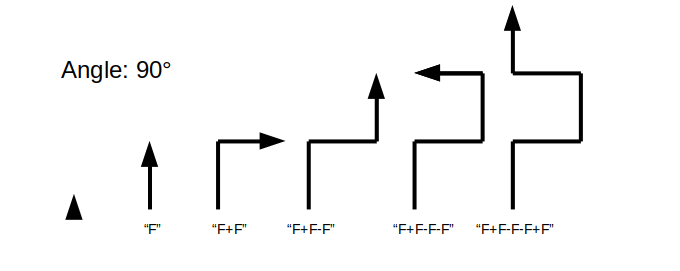
\includegraphics[scale=0.5]{Diagrams/basic_turtle.png}
		\caption{Diagram showing a turtle interpreting simple L-system string.} \label{basic turtle}
	}
\end{figure}
\FloatBarrier

\vspace{5mm}

There are a further two commands which I will be covering in detail in section \ref{branching}. We can also have constant numerical values that can be used. For instance, we could pass in a constant value of 1.0 as a parameter to the forward instruction as follows.

\vspace{5mm}

F(1.0)+F(1.0)-F(1.0)+F(1.0)

\vspace{5mm}

In doing this, we can specify that we would like to move forward by a specified amount. In this case we would like to move forward by 1.0 unit length. We will be covering parametric L-systems in detail in section \ref{parametric}.

\end{flushleft}

\section{Branching} \label{branching}

\begin{flushleft}

In the previous section there are two turtle commands in particular which were  not covered. These are the square bracket commands '[', ']'. The square bracket characters instruct the turtle object to save its position and rotation for the purpose of being able to restore that saved position and rotation later on. This allows the turtle to jump back to a previous position, facing the same direction as it was before. We can then branch off in a different direction.\\

\vspace{5mm}

A way to keep track of these saved locations, is in the form of a stack structure. Each time the '[' is called the current position and orientation of the turtle is saved to the top of the stack. While conversely when the ']' is called we restore the turtles position back to whatever position and orientation is stored on the top of the stack. \\

\vspace{5mm}

An example of this can be shown below in figure 2.2.\\

\begin{figure}[htbp]
	{\centering
		\vspace{7px}
		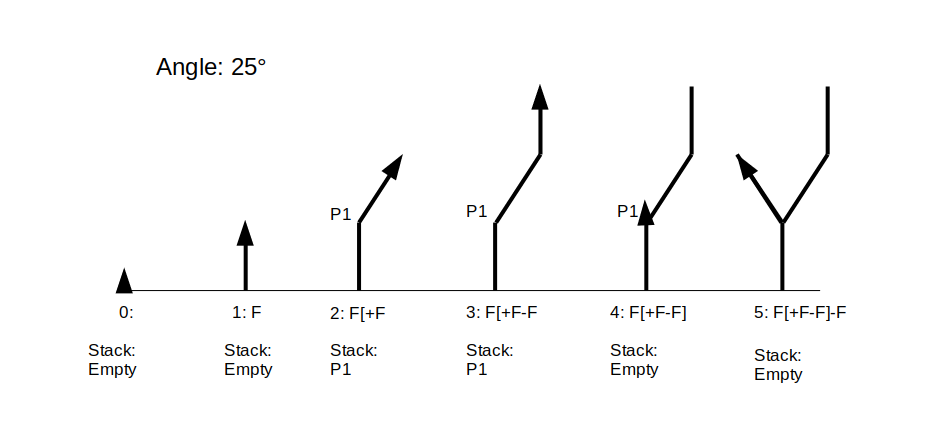
\includegraphics[scale=0.5]{Diagrams/branching_turtle.png}
		\caption{Diagram showing a turtle interpreting an L-system incorporating branching.}
	}
\end{figure}
\FloatBarrier

\end{flushleft}

\section{Parametric OL-system} \label{parametric}

\begin{flushleft}

With simplistic L-systems like the algae representation in section \ref{Simple DOL-systems} above, there are a number of details that we are not able to represent.\\
When creating a L-system to represent plants, we could assume that the width and length of each branch section is constant. We could also assume that the branching angles are also constant, 25 degrees for instance. The result of this would be that all of the important details of width and length of branches and branching angles is left up to the interpretation of the L-system string. This leaves a very large question mark as to how we should accurately interpret the L-system string. The other option would be to not only provide this information via the L-system but also to manipulate it during the re-writing process. This functionality can be provided using parametric 0L-systems set out by Prusinkiewicz and Lindenmayer. \cite{prusinkiewicz2012algorithmic} \\

\vspace{5mm}

For the purposes of this thesis we will be using the parametric L-system extensively, and we will be building some extra functionality using the concepts provided by Prusinkiewicz and Hanan \cite{prusinkiewicz1990visualization}. \\

\vspace{5mm}

\subsection{Definition of a Parametric 0L-system}

Prusinkiewicz and Hanan have defined the parametric 0L-systems as a system of parametric words, where a string of letters make up a module name $A$, each module has a number of parameters associated with it. The module names belong an alphabet $V$, therefore, $A~ \epsilon~ V$, and the parameters belong to a set of real numbers $\Re$. If $(a_1,~ a_2,~ ...,~ a_n)~ \epsilon~ R$ are parameters of $A$, the module can be stated as $A(a_1,~ a_2,~ ...,~ a_n)$. Each module is an element of the set of modules $M~ =~ V~ \times~ \Re^*$. $\Re^*$ represents the set of all finite sequences of parameters, including the case where there are no parameters. We can then infer that $M^*~ =~ (V~ \times~ \Re^*)^*$ where $M^*$ is the set of all finite modules. \\
Each parameter of a given module corresponds to a formal definition of that parameter defined within the L-system productions. Let the formal definition of a parameter be $\Sigma$. $ E(\Sigma) $ can be said to be an arithmetic expression of a given parameter. Similar to the arithmetic expressions in the programming languages C/C++, we can make use of the arithmetic operators $ +,~ -,~ *,~ \,~ \wedge{}$. The parentheses () are also used in order to specify precedence within an expression. These arithmetic expressions can be evaluated and will result in the real number parameter $\RE$.\\

The parametric 0L-system can be shown as follows as per Prusinkiewicz and Hanan's definition:\\
\\
$G~ = (V, \Sigma, \omega, P)$ 

\cite{prusinkiewicz2012algorithmic} 

\subsection{Demonstration of Parametric 0L-systems}

A parametric l-system be represented as the following: \\

\vspace{5mm}

\hspace*{3cm} n = 8\\

\vspace{5mm}

\hspace*{3cm} R 1.456\\
\hspace*{3cm} r1 85\\
\hspace*{3cm} wr 0.707\\

\vspace{5mm}

\hspace*{3cm} w : A(5)\\

\vspace{5mm}

\hspace*{3cm} p1 : A(w) : * : F(1)!(w)[/(r1)A(w*wr)][$\backslash$(r1)A(w*wr)]\\
\hspace*{3cm} p2 : F(s) : * : F(s*R)\\

\vspace{5mm}

The above l-system gives the resulting representation shown below in figure 3.8. 

\begin{figure}[htbp]
	{\centering
		\vspace{7px}
		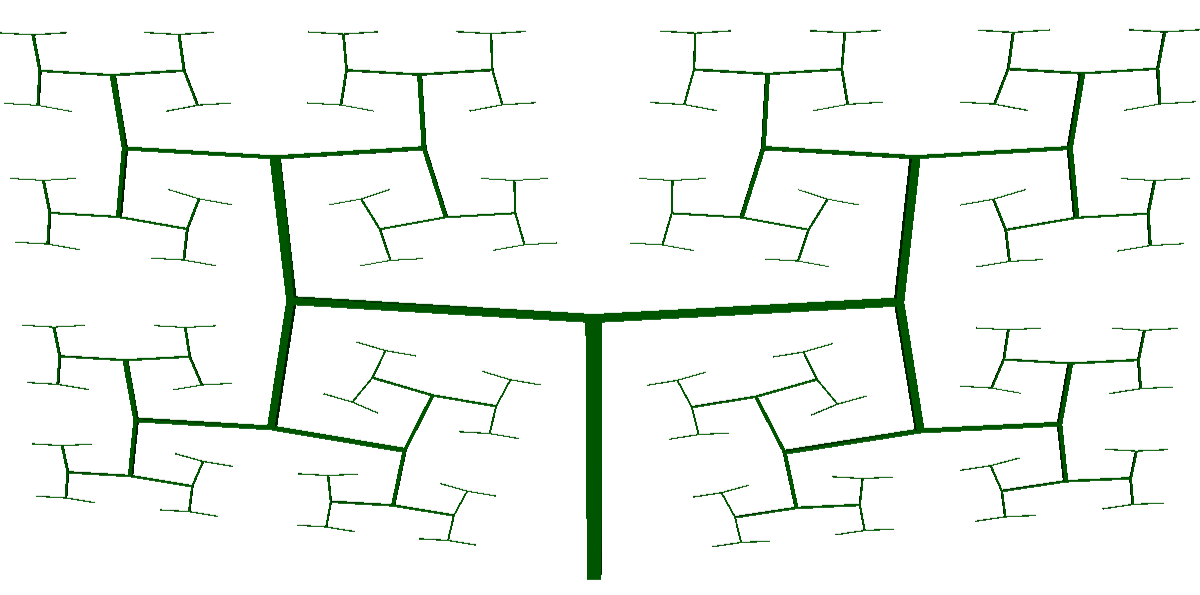
\includegraphics[scale=0.20]{ParametricLsystem/branchingPattern.png}
		\caption{3D Parametric L-system.}
	}
\end{figure}

\textit{
Defining an complex L-system grammar, with a less complexity in the interpreting system, we are given a huge amount of flexibility to define parameters that can accurately represent exactly how the L-system should be interpreted, furthermore the complexity is with the L-system grammar, so there is no need for you to make any changes to the interpreter itself. When compared to a simple L-system, you may have the advantage of being able to define simple a L-system grammar, but you would have to change and manipulate the way that the L-system is interpreted each time. Which is tedious and makes for an undesirable solution. \\
}

Similarly, to the simple DOL-systems in section \ref{Simple DOL-systems}, n refers to the number of iterations that we would like to rewrite the L-system. w refers to the Axiom string or starting states, the "\#define R 1.456" states that we are defining a constant number that will be used somewhere in the production rules or Axiom, the constant will be referred to with the name R and will have the value 1.456. \#P1, \#P2 define the production rules P1 and P2. The parametric L-system introduces the concept of a module.\\
A module is a state or variable which has zero or more parameters. The Axiom A(5) is a module with one parameter which is the number 5. A parameter can either be a number, variable or an expression of variables and numbers. For instance A(a + 1, a * b) is a valid module with the name A with two parameters a + 1 and a * b, where a and b are variables, however this is only a valid module if the value of a and b have been defined previously. Each module is treated as a single instruction, it will either be overwritten when matched with a production rule or the expression of each parameter is evaluated and is left unchanged for use when interpreted.\\
Each production rule is made up of four parts. The name, the predecessor module, the condition and the successor modules, each part is separated by a colon. Therefore the predecessor for P1 is A(w), the condition is a '*' which means that in this case there are no conditions, and the successor is F(1)!(w)[/(r1)A(w*wr)][$\backslash$(r1)A(w*wr)]. I will cover conditions in a later section.\\

\vspace{5mm}

Initially we iterate through the Axiom modules and compare them to the production rule. A match is determined if they meet three criteria.\\

\vspace{5mm}

$\bullet$ The name of the axiom module matches the name of the production predecessor. \\
$\bullet$ The number of parameters for the axiom module is the same as the number of parameters for the production predecessor. \\
$\bullet$ The condition of the production evaluates to true. If there is no condition, then the result is true by default.\\

\end{flushleft}

\subsection{Representing Randomness}

\begin{flushleft}

Randomness is an essential part of nature. If there was no randomness in plant life, we would end up with very symetric and unrealistic plants. Randomness is also responsible for creating variation in the same L-system. A L-system essentially describes the structure and species of a plant. It describes everything from how large the trunk of the tree is, to how many leaves there are on the end of branch, or even if it has flowers or not. However if there is no capability to have randomness in the generation of the L-system then we will always end up with the exact same structure. 
\vspace{5mm}
Below is a simple example of how randomness can be used to create variation.

\end{flushleft}   

\begin{figure}[htbp]
	\raggedright
	\textbf{\underline{Random Fractal:}} \\
	\#n = 2; \\
	\#w : !(0.2)F(1.0); \\
	\#p1 : F(x) : * : F(x)[+(25)F(x)][-(25)F(x)]+(\{-20.0, 20.0\})F(x)-(\{-20.0, 20.0\})F(x);\\
	\vspace{10mm}
	{\centering
		\vspace{7px}
		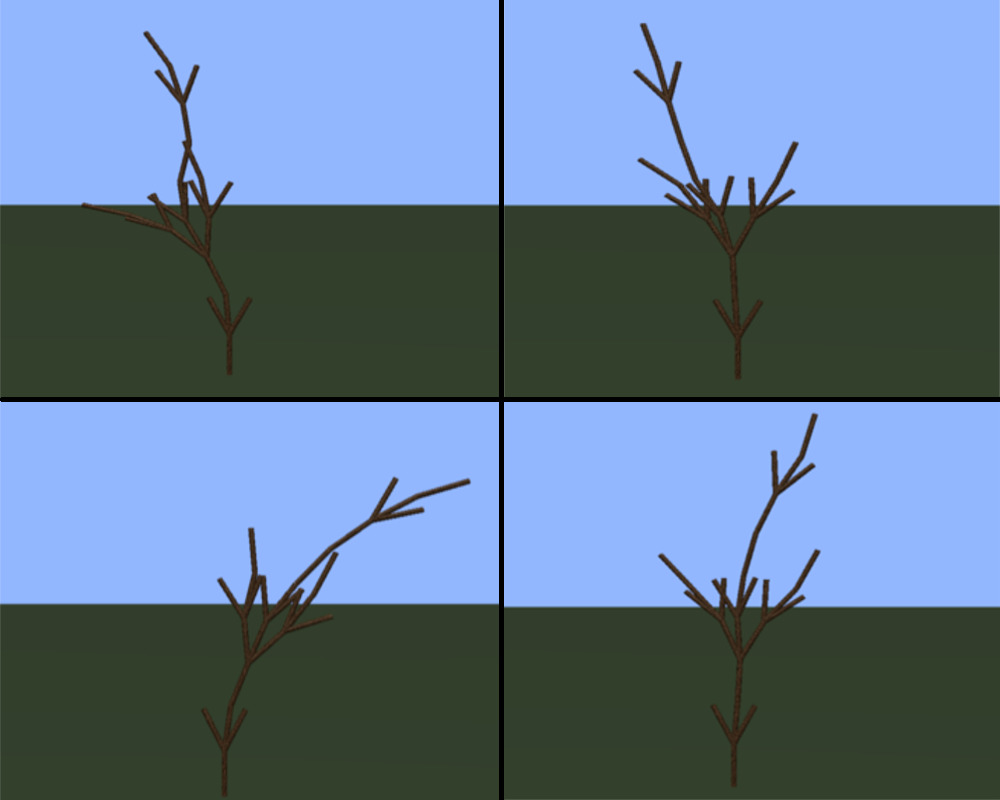
\includegraphics[scale=0.20]{Diagrams/RandomTrees.png}
		\caption{Different Variations of the Same L-system with Randomness Introduced in The Angles. \label{figRandomness}}
	}
\end{figure}
\FloatBarrier

\begin{flushleft}

In figure \ref{figRandomness} there are four variations of the same L-system using randomness, We can specify that we would like to create a random number by using the expression \{-20.0, 20.0\}. The curly braces signify that what is contained is a random number range, ranging from the minimum value as the first floating point value and the maximum value as the second floating point value separated by a comma. If both values are the same for instance +(\{10.0, 10.0\}) this is equivilant to +(10.0).

\end{flushleft}

\subsection{Representing L-system Conditions}

\begin{flushleft}

For a module to match a rule in the rule set, we need to check three criteria. The name of the rule in the predecessor matches the module name. Secondly, the number of parameters in the predecessor are the same as the number of parameters in the module. Finally, we check if the condition in the rule evaluates to true. \\

\vspace{5mm}

In this section we will be talking about the third point in the criteria above, ie., The condition must be true in order for a module to match a production rule. A condition in a rule allows us to have multiple rules that are the same in terms of the module name and the number of parameters, however they require a particalar condition to be met in order to match that rule. \\
There are six different condition operators that can be used, similar to the programming languages C/C++, as listed below.

\vspace{5mm}

$\bullet~$  '$==$'  - Equal to \\
$\bullet~$  '$!=$' - Not Equal to \\
$\bullet~$  '$>$' - Greater than \\
$\bullet~$  '$<$' - Less than \\
$\bullet~$  '$>=$' - Greater or Equal to \\
$\bullet~$  '$<=$' - Less or Equal to \\

\vspace{5mm}

The condition statement comes between the predecessor and the successor in a production rule and can be seen as an a mathematical expression on either side of the condition operator. During the rule selection process the expressions are evaluated and the results are compared using the condition operator. If the result of the condition is true then that rule is selected for rewriting, if the result is false then it moves onto the next rule. \\

\vspace{5mm}

A practical use of the condition statement might be to simulate different stages of growth. This is best illustrated using the L-system below: \\

\vspace{5mm}

\#n = 2 - 4 - 6; \\
\#object F BRANCH; \\
\#object L LEAF; \\
\#object S SPHERE; \\

\vspace{5mm}

\#define r 45; \\
\#define len 0.5; \\
\#define lean 5.0; \\
\#define flowerW 1.0; \\

\vspace{5mm}

\#w : !(0.1)I(5); \\

\vspace{5mm}

\#p1 : I(x) : x $>$ 0 : F(len)-(lean)[R({0, 100})]F(len)[R({0, 100})]I(x-1);\\
\#p2 : R(x) : x $>$ 50 : -(r)/(20)!(2.0)L(2)!(0.1); \\
\#p3 : R(x) : x $<$ 50 : -(r)$\backslash$(170)!(2.0)L(2)!(0.1); \\
\#p4 : I(x) : x $<=$ 0 : F(len)!(flowerW)S(0.3); \\

\vspace{5mm}

\begin{figure}[htbp]
\raggedright
\textbf{\underline{Random Fractal:}} \\
	{\centering
		\vspace{7px}
		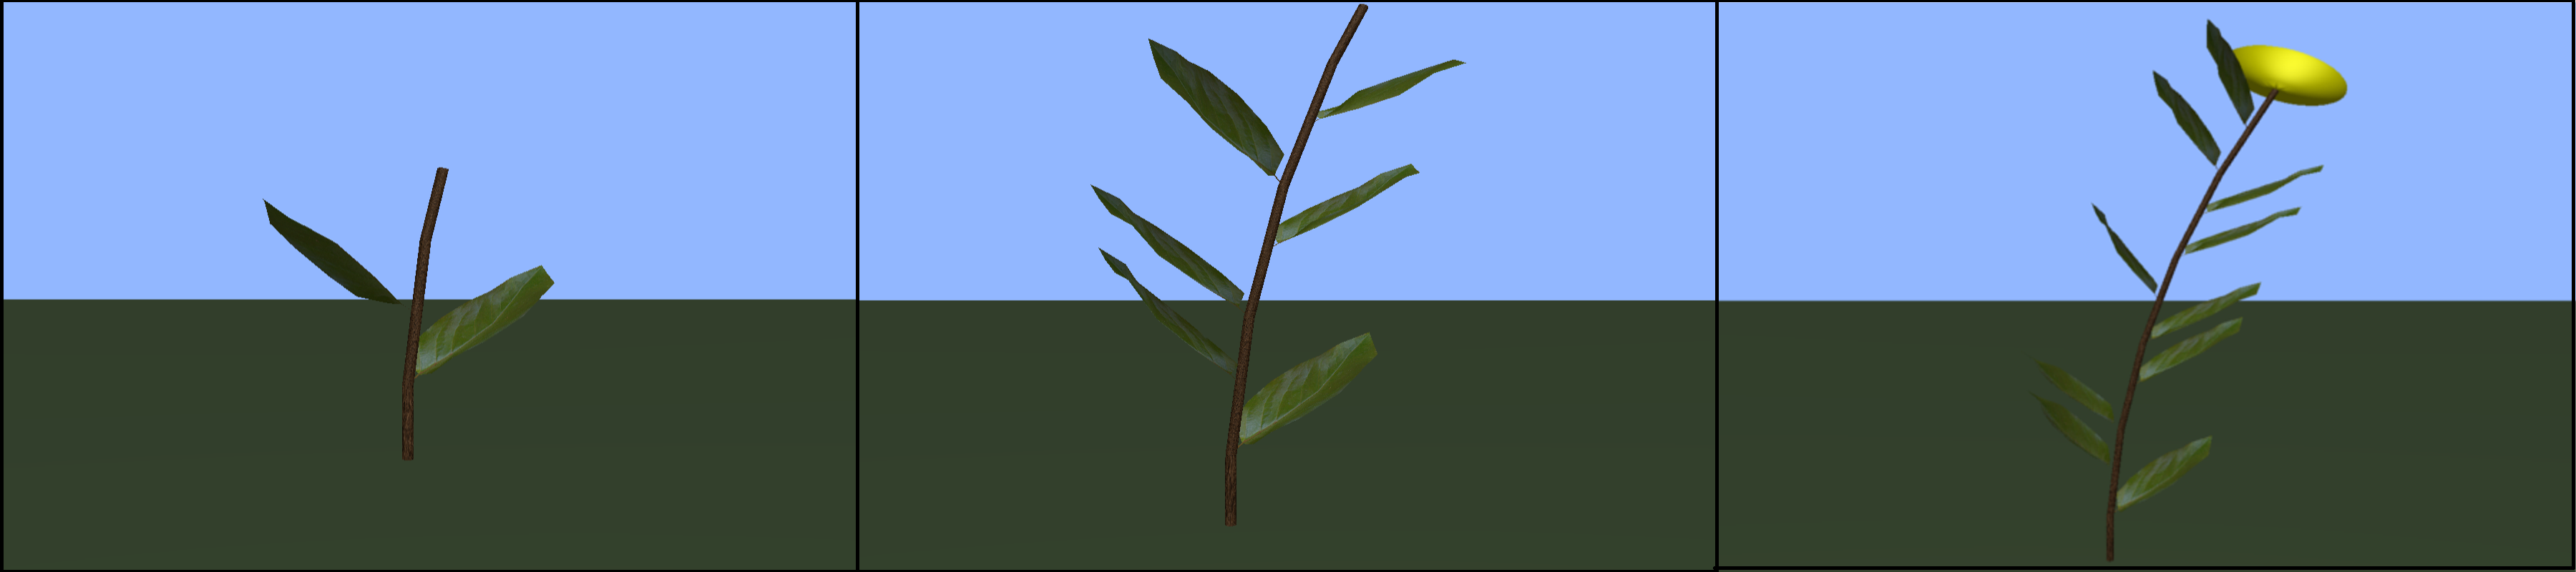
\includegraphics[scale=0.13]{Diagrams/conditionalLsystem.png}
		\caption{Condition Statements Used to Simulate the Growth of a Flower. 2nd Generation on the Left, 4th Generation in the Center and 6th Generation on the Right}
	}
\end{figure}

\FloatBarrier

\end{flushleft}

\subsection{Stochastic Rules in the L-system}

\begin{flushleft}

\begin{figure}[htbp]
	{\centering
		\vspace{7px}
		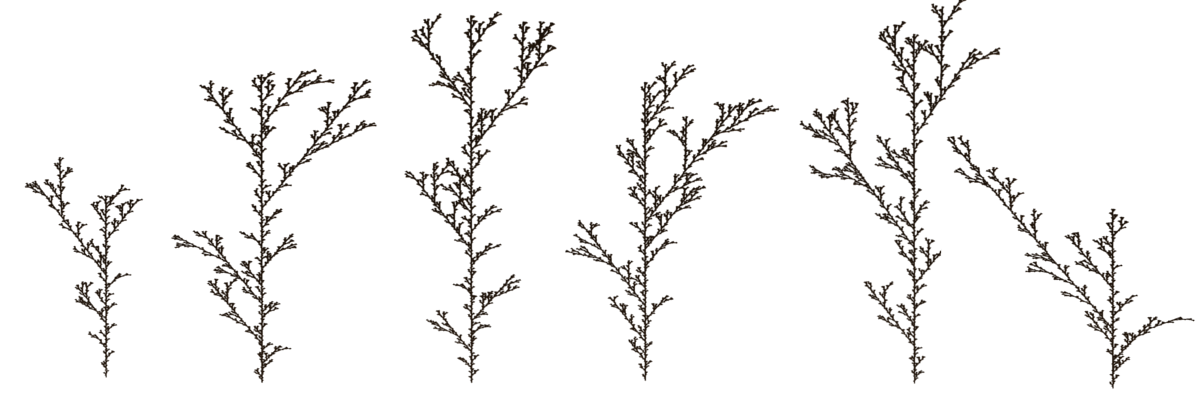
\includegraphics[scale=0.35]{Diagrams/stochastics.png}
		\caption{Representation of an L-system with a probability stochastic with a 33.33\% chance for each rule.}
	}
\end{figure}

\FloatBarrier


\end{flushleft}






